\cotefile{157-1}
\scanpage{132}
\uline{\unsure{Cofinalité}}

\mspage{$\overline{\underline{\mathrm{II}}}$}
% printed form
% margin note written sideways
\margin{MidiGraf Montpellier 21999}
% archive sheet number: 132
\scanpage{133}
\diagram{\begin{tabular}{@{}r@{\ }l@{\ }p{.65\linewidth}@{\ }l@{}}
& 1. & Mise en train (\unsure{gribouillis} \unsure{préliminaire|préliminaires}) & p. 1--10 \\
& 2. & Les cat. loc. filtrantes \unsure{''} et les cat. local.\textsuperscript{t} \unsure{str.|stric.|discr.}\textsuperscript{t} $0$-connexes (\unsure{Th.} 2.6. p. 19, prop. \unsure{2.5.} p. 14) & p. 11--36 \unsure{ter} \\
& 3. & Cofinalité et $W$-asphéricité (prop. 3.2 \unsure{page} 43\unsure{,|;} cor 3.4, p. 4\deleted{\unsure{3|5}}\unsure{5}) & p. 37--49 \\
& 4. & Foncteurs biasphériques & p. 49--68 \\
\smash{\raisebox{-.7\baselineskip}{\(\Bigg\{\)}} & 5. & \unsure{Dualité|Dualités} \unsure{formelles|formelle} (!) & p. 69--83 \\
& 6. & Transporteurs, \unsure{représentabiliseurs} \unsure{relatifs} & p. 83--89 \\
& 7. & Morphismes cofiltrants et loc. cofiltrants & p. 90--96
\end{tabular}}
% archive sheet number: 133
\scanpage{134}
% archive sheet number: 134
\diagram{\begin{tikzcd}[ampersand replacement=\&,row sep=tiny,column sep=small]
\& {}\\ {} \arrow[ur] \&\\ \& {} \arrow[ul]
\end{tikzcd}}

\diagram{\begin{tikzcd}[ampersand replacement=\&,row sep=small,column sep=small,cells={font=\scriptsize},execute at end picture={\draw (B.south west) -- (A.north east); \draw (F.south west) -- (C.north east); \draw (H.south west) -- (D.north east);}]
\& |[alias=A]| \deleted{W\text{-parfait}}\arrow[rrr,Rightarrow]\arrow[dl,Rightarrow]\arrow[dd,Rightarrow]\arrow[dr,Rightarrow] \& \& \& |[alias=C]| \deleted{W\text{-lisse}}\arrow[dl,Rightarrow]\arrow[dd,Rightarrow]\\
\deleted{W\text{-propre}}\arrow[rrr,Rightarrow]\arrow[dd,Rightarrow] \& \& \deleted{W\text{-fibr.\ faible}} \& \deleted{W\text{-net}}\arrow[dd,Rightarrow]\&\\
\& \deleted{\text{rev.}}\arrow[rrr,Rightarrow]\arrow[dl,Rightarrow]\arrow[dd,Rightarrow] \& \& \& |[alias=D]| \deleted{\text{étale}}\arrow[dl,Rightarrow]\arrow[dd,Rightarrow]\\
|[alias=B]| \deleted{\text{coétale}}\arrow[rrr,Rightarrow]\arrow[dd,Rightarrow]\&\&\&\deleted{\text{net}}\arrow[dd,Rightarrow]\&\\
\&\deleted{\text{\unsure{somme dis.} \unsure{direct}}}\arrow[rrr,Rightarrow]\arrow[dl,Rightarrow]\&\&\&\deleted{\text{imm.\ ouv.}}\arrow[dl,Rightarrow]\\
|[alias=F]| \deleted{\text{imm.\ fermée}}\arrow[rrr,Rightarrow]\&\&\& |[alias=H]| \deleted{\text{\unsure{immersions|immersion}}}\&
\end{tikzcd}}

\diagram{\(\begin{array}{l|l}\text{asph.}&\text{lisse}\\\text{coasph.}&\text{propre}\\\text{\unsure{biasp}}&W\text{-net}\end{array}\)}

\diagram{\begin{tikzcd}[ampersand replacement=\&,row sep=small,column sep=small,cells={font=\scriptsize}]
\&\text{imm.\ ouv.}\arrow[drr]\arrow[ddd]\&\&\\
\text{somm. direct}\arrow[ur]\arrow[drr]\arrow[ddd]\&\&\&\text{imm}\arrow[ddd]\\
\&\&\text{imm. ferm.}\arrow[ur]\arrow[ddd]\&\\
\&\text{étale}\arrow[drr]\arrow[ddd]\&\&\\
\text{rev. ét.}\arrow[ur]\arrow[drr]\arrow[ddd]\&\&\&\text{net}\arrow[ddd]\\
\&\&\text{coétale}\arrow[ur]\arrow[ddd]\&\\
\&W\text{-lisse}\arrow[drr]\&\&\\
W\text{-parf}\arrow[ur]\arrow[drr]\arrow[r,dashed]\&W\text{-\unsure{fibr.} faible}\arrow[rr,dashed]\&\&\unsure{\text{quelc.}}\\
\&\&W\text{-propre}\arrow[ur]\&
\end{tikzcd}}

\margin{tous les $\unsure{12-1=11|(2-1=1)}$ carrés sont cartésiens dans $\mathrm{Ens}$}

\[
\begin{aligned}
 & f : X \unsure{-|\to}Y \qquad \text{Conditions \unsure{'fines|fines}}\\
 &\left\{\begin{aligned}
\text{a)}\quad &\forall x\deleted{_{\unsure{0}}}\in X,\quad X_{/x}-Y_{/x}\quad\text{est $W$-propre}\\
\text{b)}\quad &\forall x\in X\quad {}_{x\backslash}X-{}_{y\backslash}Y\quad\text{est $W$ lisse}\\
\text{c)}\quad &\forall u:x_0-x_1\ \text{dans }X,\\
 &f_u:\underset{\backslash u/}{X}\longrightarrow\underset{\backslash\unsure{v}/}{Y}\\
 &\text{à fibres $W$-asph.}
\end{aligned}\right.
\end{aligned}
\]
Elles impliquent que les $\unsure{f_u|f}$ sont $W$-parfaits et des \unsure{$W$-univ.}. \unsure{On dit que|Qu'on dise que} $f$ est \uline{$W$-net}.

\diagram{\begin{tikzcd}[ampersand replacement=\&,row sep=small]
X\arrow[r,dash]\arrow[d]\&X'\arrow[d]\\ Y\&Y'\arrow[l,dash]
\end{tikzcd}}

\diagram{\begin{tikzcd}[ampersand replacement=\&,row sep=tiny,column sep=small,execute at end picture={\draw[rounded corners] ([xshift=-3pt,yshift=4pt]a.north west) rectangle ([xshift=4pt,yshift=-4pt]c.south east); \draw[rounded corners=8pt] ([xshift=-4pt,yshift=5pt]e.north west) rectangle ([xshift=5pt,yshift=-5pt]g.south east);}]
 |[alias=a]|0'\arrow[r]\arrow[d]\&1\arrow[r]\& 2\\
0\arrow[urr]\&\& |[alias=c]|{}\\
 |[alias=e]|0\arrow[r]\&1\arrow[r]\& |[alias=g]|2
\end{tikzcd}}
% slanted
\margin{$\Downarrow$ \unsure{morphisme} $W_{\unsure{\infty|w}}$-lisse à fibres $W_{\infty}$-asph, mais non $W_{\infty}$-net ni \unsure{$\Leftrightarrow$|a fortiori} $W_0$-net car $\,{}_{0'\backslash}X_{/2}\to{}_{0\backslash}Y_{/2}$ a une fibre en $1$ \unsure{$\simeq$} vide \unsure{$\hookleftarrow$}.}

\uline{Question}\ \tikz[baseline]{\draw[->] (.50em,-.08em) to[out=115,in=0] (-.30em,.68em);} Si $f$ $W$-lisse (resp $W$-propre), est-il $W$-net ? \tikz[baseline=(nn.base)]{\node[draw,ellipse,inner sep=1pt] (nn) {Non};} Mais si $f$ $W$-parfait ???
\scanpage{135}
\diagram{\begin{tikzcd}[ampersand replacement=\&,row sep=small,column sep=small]
X\arrow[dd]\&\&X'\arrow[ll]\arrow[dd]\&\\
\&X_{/y}\arrow[ul]\arrow[dd,"\text{coasph.}"]\&\&X'_{/y'}\arrow[ll]\arrow[ul]\arrow[dd,"\text{coasph. ?}"]\\
Y\&\&Y'\arrow[ll,"{\deleted{\text{\unsure{lisse}}}}"]\&\\
\&Y_{/y}\arrow[ul]\&\&Y'_{/y'}\arrow[ll,"{\substack{\deleted{\text{lisse à fibres}}\\\text{asph.}}}"]\arrow[ul]
\end{tikzcd}}

Catégories sur $\Delta^2$ (\unsure{motivé} par question du \unsure{composé|comportement} des $W^{\unsure{u|n}}$)

\diagram{\begin{tikzcd}[ampersand replacement=\&,row sep=small,column sep=small,execute at end picture={\draw ([xshift=-6pt,yshift=7pt]a.north west) to[out=0,in=85] ([xshift=5pt]b.east);}]
|[alias=a]|X_0\arrow[dr,dash,"{\substack{\text{coét}\\\text{asph.}\\\text{i.e iso}}}"'] \&\\ \&|[alias=b]|X_1
\end{tikzcd}}

\diagram{\begin{tikzcd}[ampersand replacement=\&]
X\&\\ {}\arrow[r,very thick]\&{}
\end{tikzcd}}

\diagram{\begin{tikzcd}[ampersand replacement=\&,row sep=small,column sep=small]
X\arrow[d,"\text{coasph.}"']\&X'\arrow[l]\arrow[d,"\text{coasph. ?}"]\&\\
Y\&Y'\arrow[l,"{\substack{\text{lisse}\\\text{à fibres}\\\text{asph.}}}"]\&\\
{}_{y\backslash}Y\arrow[u]\&\&{}_{y'\backslash}Y'\arrow[ul]\arrow[ll]
\end{tikzcd}}

\[
\begin{aligned}
 &\deleted{\unsure{\Delta^2}}\\
 &X_{01}\qquad X_{12}\qquad X_{02}
\end{aligned}
\]

\diagram{\begin{tikzcd}[ampersand replacement=\&,row sep=small,column sep=small]
\&X_1\arrow[dr]\&\\
\unsure{\alpha|X}_{01}\arrow[ur,dash]\arrow[dd,leftrightarrow,"\unsure{a}"]\&\&X_{12}\\
\&\deleted{\unsure{X}}\arrow[uu]\arrow[dl]\arrow[dr]\&\\
X_0\arrow[dr]\&\&X_2\arrow[uu]\arrow[dl]\\
\&X_{0,\unsure{2}}\&
\end{tikzcd}}

\figure{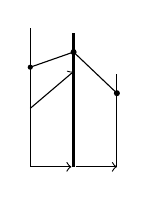
\begin{tikzpicture}[scale=.55]
\draw (0,0)--(0,3.2); \draw[very thick] (1,0)--(1,3.1); \draw (2,0)--(2,2.15);
\draw[->] (0,0)--(.95,0); \draw[->] (1.05,0)--(2,0);
\draw (0,2.3)--(1,2.65)--(2,1.7); \draw[->] (0,1.35)--(1,2.2);
\fill (0,2.3) circle (.06) (1,2.65) circle (.07) (2,1.7) circle (.07);
\end{tikzpicture}}

\diagram{\begin{tikzcd}[ampersand replacement=\&,row sep=small,column sep=small,cells={font=\scriptsize}]
\&\overset{\text{asph.}}{X_{02}}\arrow[dd,"W"]\&X_2\ \text{asph}\arrow[l,"{\deleted{\unsure{W}}}"]\arrow[dd,"W"]\\
\text{asph. }X_0\arrow[ur,"\text{asph}"]\arrow[dd,"\text{asph}"']\&\&\\
\&\underset{\text{asph.}}{X_{012}}\&X_{12}\ \text{asph}\arrow[l,"W"]\\
\text{asph }X_{01}\arrow[ur,"W"]\&\&\\
\&\underset{\text{asph.}}{X_1}\arrow[ul,"W"']\arrow[uur,"\text{asph.}"']\&
\end{tikzcd}}

\diagram{\begin{tikzcd}[ampersand replacement=\&,row sep=small,column sep=small,cells={font=\scriptsize},execute at end picture={\draw ([xshift=-4pt,yshift=2pt]z.north west) -- ++(0.65,1.8);}]
\&\&\&\&\widetilde X_{0\unsure{2|7}}\arrow[dddd,bend left=45]\\
\&\&\overset{\text{asph}}{\widetilde X'_{02}}\arrow[urr]\arrow[ddl,"\text{\unsure{Catfib}}"']\arrow[ddr,leftrightarrow,"{\text{\unsure{Catcof}}}","{\underline{\text{asph}}}"']\&\&\\
\&\&\&\&\\
\&\text{asph. }\widetilde X_{01}\arrow[dl,"\text{\unsure{Catfib}}"']\arrow[dr,"{\text{Cof}}","{\underline{\text{asph}}}"']\&\&\widetilde X_{12}\ \text{asph.}\arrow[dl,"\text{fib}"']\arrow[dr,"{\text{\unsure{Catcof}}}","{\underline{\text{asph}}}"']\&\\
|[alias=z]| \underset{\text{asph}}{X_0}\&\&\underset{\text{asph}}{X_1}\&\&\underset{\substack{\text{asph,}\\\text{(objet final)}}}{X_2}
\end{tikzcd}}
% archive sheet number: 135
\scanpage{136}
\mspage{PU 51}

\margin{\handwritten{\unsure{$\times$|*}}}\inserted{\handwritten{à}} quelles fins...), parmi d'autres structures, d'une soi-disante structure de graphe (dite ``structure d'affinité''), sans qu'il soit trop sûr à aucun moment si telle paire de sommets représente bien ``une arête'' (i.e. si ses deux termes sont considérés ``voisins''), ou non !

Mais une telle situation ne semblera pas tellement étrange au mathématicien \margin{\handwritten{*}}(disons) qu\deleted{\unsure{e}}\handwritten{i} serait rompu à la tâche d'édifier des théories, où les n o t i o n s même avec lesquelles on sera amené à travailler restent encore dans les limbes du non-cré\leavevmode\rlap{e}\handwritten{\'{\phantom{e}}}. Il s'agit\unsure{,}alors de les tailler sur pièces justement, une à une et patiemment, pour arriver à donner un sens à quelque informe nuage d'intuitions, lesquelles peuvent toutes sembler évanescentes et impalpables, mais dont on s e n t pourtant, avec une ``évidence'' pour ainsi dire charnelle et au delà de tout doute, une texture tangible et une chaude substance.

C'est le non-né alors qui nous souffle à chaque moment, au fur et à mesure que le travail de la naissance progresse, quelle doit être telle portion de forme qui s'apprête à naître, et par quel bout la prendre pour la voir émerger du néant et ê t r e. Le tâtonnement même de la main qui saisit la chose encore non née pour l'amener au jour, n'est indécision ni errance, mais prise de connaissance d'où toute hésitation, toute perplexité est absente.

Et ces choses que nous écrivons comme si u n\quad a u t r e écrivait par notre main, et que nous croyons apprendre en les écrivant - quelque part en nous, en des profondeurs ignorées, elles étaient s u e s déjà bien avant que notre main ne les écrive, et n'attendaient que l'attention intense du s c r i b e à l'écoute, qui veuille bien les consigner.

16. La Fleur et son mouvement - ou : plus je m'éloigne, plus je m'approche

(25 mars) Quelques commentaires encore sur notre fleur cosmique, avant de la quitter pour poursuivre le fil interrompu de la réflexion.

Les douze termes yang, placés sur le cercle extérieur, forment aussi les point\deleted{s}\handwritten{es} des douze pétales de la corolle : \deleted{\unsure{c|C}}\handwritten{\unsure{c|C}}eux-ci se rejoignent deux par deux, en les douze points d'insertion sur le cercle intérieur, figurant les douze termes yin de l' ``harmonium''.

Chaque pétale, regardé séparément, se présente aussi comme une sorte de ``mont'' de forme ogivale, dont le sommet yang forme couple avec chacun des deux termes yin, représentés par les points les plus bas\inserted{\handwritten{(*)}} de l'un et l'autre versant du mont. Ces points marquent en même temps le fond des ``vallées'', ou ``ravins'',

\handwritten{(*) Il est entendu ici que la direction vers le ``bas'' est celle vers le centre de la Fleur cosmique.}
% archive sheet number: 136
\scanpage{137}
\diagram{\begin{tikzcd}[ampersand replacement=\&,column sep=small,row sep=small,cells={font=\scriptsize}]
\&\&X_0\arrow[d,leftrightarrow]\&\&\\
\&\&\widetilde X_{02}\arrow[dll,"\text{fib}"']\arrow[drr,"{\text{cof, }W_{\unsure{\mathrm{univ}}}}"]\&\&\\
X_0\arrow[dd,leftrightarrow,"\text{fib}"']\&\&\&\&X_2\ni e_2\arrow[dd,leftrightarrow,"{\text{cof, }W_{\mathrm{univ}}}"]\\
\&\&\widetilde X^{\prime\unsure{+}}_{02}\arrow[uu,"(W)"]\arrow[dll,"\text{fib}"']\arrow[drr,"{\text{cof, }W_{\mathrm{univ}}}"]\arrow[ull,dotted,dash]\arrow[urr,dotted,dash]\arrow[dd,dotted,dash,"{\substack{x_{02}\\[-2pt]\diagup\ \diagdown\\[-2pt]x'_{01}\quad x'_{12}\\\text{cart}}}"]\&\&\\
\widetilde X_{01}\arrow[drr,"{\substack{\text{cof}\\ W_{\mathrm{univ}}}}"']\&\&\&\&\widetilde X_{12}\arrow[dll,"\text{fib}"]\\
\&\&X_1\&\&\&\unsure{x|X}_1\arrow[ul,leftrightarrow]
\end{tikzcd}}

\diagram{\begin{tikzcd}[ampersand replacement=\&,execute at end picture={\foreach \x in {0,.15,.30,.45}{\draw ([xshift=\x cm,yshift=-5pt]a.south) -- ([xshift=\x cm,yshift=5pt]b.north);}}]
\& |[alias=b]| \deleted{\unsure{1}}\arrow[r]\&\deleted{2}\\
 |[alias=a]| \deleted{0}\arrow[ur]\arrow[urr,bend left]\arrow[urr,bend right]\&\&
\end{tikzcd}}

\diagram{\begin{tikzcd}[ampersand replacement=\&,row sep=small,column sep=small]
\&1\arrow[r]\&2\\0\arrow[ur]\arrow[urr]\arrow[d,leftrightarrow]\&\&\\0'\arrow[uurr]\&\&
\end{tikzcd}}

\[
 X_0^{\unsure{0|\circ|o}}\longrightarrow\unsure{\mathrm{Co\acute et}}(X_1)
\]
\[
\begin{array}{l|l}
X_0\ \text{asph.} &X_0\unsure{-|\to}X_{01}\ \text{asph.}\\
X'_{01}\ \text{asph.}&\deleted{\text{\unsure{mais}}}\ X_0,X_1\ \text{asph.}\\
\text{mais}&\deleted{\text{mais}}\ X_1\to X_{01}\ \text{pas asph.}\\
&\text{i.e.}\quad X_{01}-\Delta^1\quad\text{lisse }\deleted{\text{à fibr}}\ \inserted{W_{\mathrm{univ}}},\\
&\hfill\deleted{\text{mais}}\ \text{\uline{pas} propre}
\end{array}
\]
\[
\begin{aligned}
 &\deleted{\unsure{X_0\longrightarrow(X_1^\vee)}}\\
 &X_1\longrightarrow(X_0^\wedge)_{\text{asph.}}
\end{aligned}
\]

\diagram{\begin{tikzcd}[ampersand replacement=\&,row sep=tiny,column sep=tiny,execute at end picture={\foreach \s in {0,2,4,6,8}{\draw ([xshift=\s pt]lo.west) -- ([xshift=\s pt]hi.north west) -- ([xshift=\s pt]lo.center);}}]
\&0\arrow[r,very thick]\arrow[d]\&\cdot\arrow[r]\&\bullet\&\\
|[alias=hi]| \deleted{\unsure{0}}\arrow[r]\arrow[d,dash]\&\underset{\unsure{1}}{\cdot}\arrow[urr]\&\&\&{}\arrow[d,dash]\\
|[alias=lo]|{}\arrow[r,very thick]\&\underset{0}{\bullet}\arrow[r,very thick]\&{}\arrow[r]\&{}\&{}
\end{tikzcd}}
$W_{\unsure{\infty|w}}$-lisse ? non $W_0$-propre non $W_0$-net.

\deleted{\unsure{$f$}}\quad $W$-parfait $\overset{?}{\Longrightarrow}$

\diagram{\begin{tikzcd}[ampersand replacement=\&,row sep=tiny,column sep=tiny]
\&1\arrow[dr]\&\\0\arrow[ur]\arrow[dr]\&\&2\\ \&1'\arrow[ur]\&\\
0\arrow[r]\arrow[uu,leftrightarrow]\&1\arrow[r]\&2
\end{tikzcd}}

\diagram{\begin{tikzcd}[ampersand replacement=\&,row sep=tiny,column sep=tiny]
0\arrow[r]\arrow[d]\&1\arrow[r]\&2\arrow[d,very thick]\\
0'\arrow[urr,very thick]\arrow[rr,"{\deleted{\unsure{-}}}"']\&\&2'\\
0\arrow[r]\&1\arrow[r]\&2
\end{tikzcd}}

\diagram{\begin{tikzcd}[ampersand replacement=\&,row sep=tiny,column sep=tiny]
\&{}\arrow[d]\&\\
{}\arrow[d]\arrow[r,very thick]\&{}\arrow[r,very thick]\&{}\\
{}\arrow[rr,very thick]\&\&{}\arrow[u]\\
{}\arrow[r]\&{}\arrow[r]\&{}
\end{tikzcd}}
\[
\begin{aligned}
 &\deleted{\unsure{X_{/x}\longrightarrow Y}}\qquad X\longrightarrow\Delta^2\\
 &X_{/x}=
\end{aligned}
\]
% archive sheet number: 137
\scanpage{138}
\mspage{PU 50}

Le même terme peut être yang dans sa relation à tel autre, et yin dans sa relation à tel autre encore. Voir à ce sujet la section ``L'ambiguité créatrice (1) : paires, ribambelles et rondes'' (n° 3).

\noindent\rule{8em}{.4pt}

Comme je l'ai souligné dès le début de cette réflexion, il semble bien qu'une fois choisi l'ensemble $\mathrm T$ des ``termes'', représentant les qualités et entités cosmiques qu'on se propose d'étudier, la structure de graphe orienté correspondante est déterminé sans ambigu\leavevmode\rlap{i}\handwritten{\"{\phantom{\i}}}té. C'est-à-dire, pour deux termes $\mathrm a$ et $\mathrm b$ dans $\mathrm T$, on peut décider (par une intuition ou une réflexion de nature ``philosophique'', visiblement extra-mathématique) si ces deux termes ``forment couple'', et si oui, lequel des deux termes y joue le rôle yang (ou encore, doit figurer comme ``origine'' de l'arête orientée joignant les deux sommets représentatifs de $\mathrm a$ et de $\mathrm b$).

La deuxième structure qui est intervenue jusqu'à présent, se superposant à la première, est la structure d' a f f i n i t é. En langage mathématique courant, c'est encore une structure de g r a p h e (mais non orienté cette fois), consistant dans la prescription, parmi l'ensemble de toutes les ``paires'' possibles d'éléments de $\mathrm T$ (i.e. de parties de $\mathrm T$ réduites à deux éléments $\mathrm a,\ \mathrm b$), d'un certain sous-ensemble, formé des paires $\{\mathrm a,\mathrm b\}=\{\mathrm b,\mathrm a\}$ pour lesquelles $\mathrm a$ et $\mathrm b$ sont considéré\deleted{e}s comme étant ``voisins'', ou comme ``présentant des affinités''. Cette notion d'affinité est, elle aussi, de nature ``philosophique'', mais cette fois beaucoup moins clairement définie. Il n'y aura guère de lecteur qui ne décèlera, sans nuance d'une hésitation, un ``affinité'' entre ``rêve'' et ``imagination'', ou entre ``rêve'' et ``le possible''. Par contre, la question si ``rêve'' est voisin de ``hasard'', ou de ``jeu'', voire de ``liberté'' ou d' ``abandon'', aura sûrement des réponses bien différentes d'une personne à l'autre, et même chez la même personne, suivant les dispositions dans lesquelles elle abordera cette question. En fait, ce que nous révèle une intuition philosophique plus ou moins exercée, ce n'est pas tant une information du type ``tout ou rien''(``$\mathrm a$ et $\mathrm b$ sont voisins'', ou : ``ils n'ont rien à voir'') mais plutôt du type ``plus ou moins'' (comme : ``$\mathrm a$ et $\mathrm b$ sont très voisins'', ou ``assez voisins'', ou ``vaguement apparentés''...). C'est ce ``vague'' indissociable, semblet-t-il, de la notion d'affinité (dans le contexte qui nous intéresse), qui est cause aussi de l'arbitraire que je signalais dès le début, pour la formation des ``groupes'' de couples et des ``affinités'' entre tels groupes, par quoi former le diagramme (non orienté) des ``portes sur l'Univers'', alias ``diagramme en arbre de Noël''.

On est donc dans une situation un peu de guingois, où le mathématicien habitué à travailler avec des structures bien définies, se verrait confronté à une \margin{\handwritten{\unsure{$\times$|*}}}sorte de ``structure floue'', où il est censé tirer partie (\deleted{à} on ne\deleted{\unsure{l'|y}} sait trop encore
% archive sheet number: 138
\scanpage{140}
\[
\begin{aligned}
\mathbb N\deleted{_{\unsure{x}}}&\longrightarrow I: \\[-2pt]
&\phantom{\longrightarrow}\{i\}
\end{aligned}
\]
\[
 I\longrightarrow\unsure{\mathscr D|\mathscr O}.
\]
\[
\left.\begin{aligned}
 &\unsure{\mathbb I|I}\ \text{filtrante finie}\\
 &\mathbb N\longrightarrow I
\end{aligned}\right\}\quad
\begin{aligned}
 &\text{alors $I$ est grand devant $\pi$}\\
 &\text{pour tt cardinal $\pi$}
\end{aligned}
\]
\deleted{\unsure{car pour tt} \illegible{1}}

\uline{Prop} Soit $I$ une catégorie équiv. à une petite cat. Conditions équivalentes, soit $\pi_0=\operatorname{card}\operatorname{Fl} I$

a) $I$ est grand devant $\pi$ pour tt card $\pi$

b) $I$ est grand devant $\pi'_0=\operatorname{Sup}(\pi_0,\aleph_0)$ (i.e. \unsure{$I$ grand} devant $\pi_0$, si $\pi_0$ est infini)

c) Il existe un foncteur cofinal $I'\longrightarrow\mathbb I$, où $I'$ est une catégorie \unsure{filtrante} finie.

d) \deleted{Il existe un foncteur \unsure{cofinal} $I'$} \inserted{comme c), \unsure{sauf|avec|mais} $I'$ \deleted{\unsure{étant}} la cat.} $I^{\unsure{*}}_0$ réduite à un seul objet, avec une seule flèche non identique $\unsure{p|\rho}$, satisfaisant $p^2=p$.

e) Il existe un objet $x_0$ de $I$, et une section de $x_0$ sur l'objet final $e_{I^\wedge}$ de $I^\wedge$ -- i.e. pour tt $x\in\operatorname{Ob} I$, un $x\xrightarrow{f_x}x_0$ tel que .... \unsure{sinon pas}.

\deleted{\unsure{réciproquement} \illegible{2}}
\diagram{\begin{tikzcd}[ampersand replacement=\&,row sep=small,column sep=small]
\deleted{a}\arrow[r,Rightarrow]\&\deleted{\unsure{b}}\arrow[r,Rightarrow]\&\deleted{\unsure{c}}\arrow[r,Rightarrow]\&\deleted{\unsure{d}}\\
\deleted{c}\arrow[r,Rightarrow]\&\deleted{\unsure{a}}\arrow[r,Rightarrow]\&\deleted{b}\&
\end{tikzcd}}
\margin{\deleted{\unsure{démonstration}} pour une cat. finie}
\diagram{\begin{tikzcd}[ampersand replacement=\&,row sep=small,column sep=small]
\&\&\&\&c\\
e\arrow[r,Leftrightarrow]\&d\arrow[r,Rightarrow]\&a\arrow[r,Rightarrow]\&b\arrow[ur,Rightarrow]\arrow[r,Rightarrow]\&e
\end{tikzcd}}
\margin{$\downarrow$ \unsure{exc.|exerc.} \unsure{dét.|déterm.} des foncteurs cofinaux $I_0\to I$}
\margin{$\searrow$ \deleted{\unsure{tr}} \unsure{triv.}}
\[
\begin{aligned}
 &\unsure{\text{donc}}\ e\Longleftrightarrow d\Longleftrightarrow a\Longrightarrow b\\
 &\deleted{\unsure{b\Longrightarrow}}\Longrightarrow c
\end{aligned}
\]
\margin{\deleted{\unsure{on}} \unsure{Appliquant|Appliquer} ceci au cas d'une catégorie \deleted{finie} $I'$, on trouve \deleted{\unsure{que}} \deleted{\unsure{b}} $c\Rightarrow d$ dans tt cat équiv. \unsure{une}}

\diagram{\begin{tikzcd}[ampersand replacement=\&,row sep=small,column sep=small]
{}\arrow[r,shift left=1.2ex]\arrow[r,shift left=.4ex]\arrow[r,shift right=.4ex]\arrow[r,shift right=1.2ex]\&x\arrow[r,"p"]\&\deleted{\unsure{x}}
\end{tikzcd}}
\[
\begin{aligned}pu&=u\\p^2&\deleted{\unsure{\ne}}=p\end{aligned}
\]
% margin note written upside down
\diagram{\begin{tikzcd}[ampersand replacement=\&,row sep=small,column sep=small]
\&\underline S(\unsure{\pi|\mathbb I})_{/x}\arrow[d,"\text{cofinal}"]\\
J\arrow[ur,bend left=14,"{\deleted{\text{4.4.2}}}"]\arrow[r,"{\deleted{\text{cof}}}","{\substack{\text{cof.}\\\text{par }4.4.2.}}"']\&\mathcal M_{\pi/x}
\end{tikzcd}}
% archive sheet number: 140
\scanpage{141}
Papier brouillon (pour \unsure{Jordano|Jordens} ?)

\diagram{\begin{tikzcd}[ampersand replacement=\&]
\unsure{\mathscr J|J}\arrow[r,"\text{cof. ?}"]\arrow[dr,dashed]\&\mathscr J^B\arrow[d,"\text{cof ?}"]\\
I\arrow[u,"\text{cof}","{\text{pl fid}}"']\arrow[r,"\text{cof}"]\&I^B
\end{tikzcd}}
\margin{4.\unsure{9|4}.6.3. 2° p. \unsure{284--285|224--225}}

\[
\begin{aligned}
 &J\hookrightarrow I\\
 &\text{pl fid. cofinal}\qquad &\unsure{\not\Longrightarrow|\longmapsto}\quad J\ \text{grand devant }\pi\\
 &I\ \text{grand devant }\pi &&\text{OK}\ \unsure{\text{pour}}.
\end{aligned}
\]
\[
 \unsure{i|1}\rightrightarrows f(j)\longrightarrow\unsure{j'|y'}\longrightarrow f(j')
\]
\[
 \mathop{\mathrm{Card}}\alpha_0\leq\pi
\]
\[
 \deleted{J_0\quad J_1\quad J_2\quad\unsure{\cdots}\quad J_{\alpha}}
\]
\[
 J=\mathscr J_1\cap J_2\qquad\deleted{\unsure{\bigcap}}\quad\deleted{\unsure{J_\alpha}}
\]
$\operatorname{card} A=\unsure{\lambda^{\leq\pi}|\lambda\leq\pi}$ ($\alpha_\lambda$ plus petit ordinal de \unsure{cardinal} \unsure{$\lambda|\alpha$})

\figure{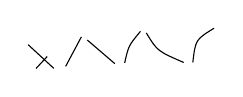
\begin{tikzpicture}[scale=.5]
\draw (0,.6)--(.65,0); \draw (.2,0)--(.48,.3); \draw (.95,.05)--(1.35,.8);
\draw (1.5,.72)--(2.2,.12); \draw (2.45,.14)..controls(2.55,.58)..(2.85,.94);
\draw (3,.9)..controls(3.28,.44)..(3.95,.15); \draw (4.18,.15)..controls(4.25,.73)..(4.72,1.02);
\end{tikzpicture}}
\[
 \operatorname{card}A\leq\pi
\]
$\alpha_0$ premier ordinal de cardinal \deleted{\unsure{$\leq$}} $\pi$

$I_{\alpha_0}\longrightarrow A$ tel que pour tt \deleted{\unsure{surjectif}} $r\in A$, $\varphi^{-1}(r)$ cofinal dans $\unsure{\mathbb I|I}_{\alpha_0}$ \unsure{i.e.|ou} $\operatorname{card}\varphi^{-1}(r)=\pi$
% archive sheet number: 141
\scanpage{143}
\mspage{1}
1. \uline{Cofinalité} \uline{cohomologique}

Soit
\[
 \alpha:C'\longrightarrow C
\]
un foncteur de (petites) Catégories, $M$ une catégorie ayant des $\varprojlim$ \unsure{pertinentes}, $F$ un préfaisceau\inserted{\unsure{donc contravariant ici}} sur $C$ à val. dans $M$. On a \unsure{un hom.|une trans.} can. dans $M$
\[
 \varprojlim_C F\longrightarrow\varprojlim_{C'}\underbrace{\alpha^*(F)}_{F\circ\alpha}
 \tag*{(1)}
\]
et \uline{\unsure{Ch.|Cher.}} \deleted{\unsure{cond}} des conditions sur $\alpha$ pour que ce soit tjrs un iso. On est ramené aussitôt au cas de $M=(\mathrm{Ens})$.
% slanted
\margin{On dit alors que $\alpha$ est \uuline{cofinal}, cf SGA 4, \unsure{4 I|I} \S~8.1. ou 3.3. p. 45}
\deleted{On dit \unsure{parfois que} $\alpha$ est \unsure{cofinal} si pour tt \unsure{$x$}} \deleted{On a \unsure{$C$}}

Disons qu'une catégorie $\unsure{\mathbb I|I}$ est \inserted{\uline{fbt}} \uline{filtr. à g} si \inserted{$I\ne\varnothing$ et} si $\forall\,\unsure{i'|x'},\unsure{i''|x''}\in\operatorname{Ob}I$, $\exists\,i\in\operatorname{Ob}I$ et des flèches
\diagram{\begin{tikzcd}[ampersand replacement=\&,row sep=small,column sep=small]
\&i'\\i\arrow[ur]\arrow[dr]\&\\ \&i''
\end{tikzcd}}
Cela signifie aussi que $\operatorname{Ob}I$ en tant qu'ens ordonné est filtrant à gauche.

\uline{Proposition} Pour que (1) soit toujours un iso, \inserted{($\alpha$ ``anodin pour $\varprojlim$'')} il suffit que pour tout $x_0\in\operatorname{Ob} C$, la catégorie ${}_{x_0\backslash}\overset{\vee}{C'}^{\unsure{x_0|y_x}}$ des couples $(x',u)$, avec $x'\in\operatorname{Ob}C'$, $u:\alpha(x')\longrightarrow x_0$, soit fbt. filt. à g.
% slanted
\margin{\unsure{cf condition bien|amélioration bien} \unsure{moins que|moins exigeante} p. 5. \quad cf 3.2 p. 43--44 pour \unsure{caractérisation|condition} de cofinalité}

Ceci n'implique pas la conclusion plus forte
\[
 F\xrightarrow[\mathrm{adj.}]{\sim}\alpha_*\alpha^*F
\]
que le morphisme d'adj. canonique soit un iso. Pour qu'il en soit ainsi, il \deleted{faut} \inserted{suffit} que $\forall x_0\in C$, le foncteur \inserted{$\alpha_{/x_0}:$} $C'_{/x_0}\unsure{-|\to}C_{/x_0}$ induit par $\alpha$ soit ``anodin pour les $\varprojlim$'', ce qui signifie aussi que pour toute flèche $u:x_1\longrightarrow x_0$ dans $C$, la catégorie $\underset{u}{\underset{\vee}{C'}}$ formée des triplets $(x',\zeta,\eta)$ avec $x'\in\operatorname{Ob}C'$ et $\zeta:x_1-\alpha(x')$, $\eta:\alpha(x')\longrightarrow x_0$ rendant commutatif
% archive sheet number: 143
\scanpage{144}
\mspage{2}
le diagramme
\diagram{\begin{tikzcd}[ampersand replacement=\&,column sep=small]
\deleted{\unsure{y|x}}x_1\arrow[rr,"u"]\arrow[dr,"\zeta"']\&\&x_0\\
\&\alpha(x')\arrow[ur,"\eta"']\&
\end{tikzcd}}
est \inserted{fbt} filtrante à g.

plus généralement, considérons
\diagram{\begin{tikzcd}[ampersand replacement=\&]
X'=C'\arrow[rr,"\alpha"]\arrow[dr,dash,"f'"']\&\&C=X\arrow[dl,dash,"f"]\\
\&S\&
\end{tikzcd}}
et posons nous la question quand la \unsure{flèche|formule} \unsure{fonctorielle}, par rapport à un préfaisceau $F$ \inserted{variable} sur $X$,
\[
 f_*(F)\longrightarrow f'_{\unsure{*|d}}(\alpha^*(F))
\]
est toujours un iso. (Le cas précédent est celui où $\deleted{\unsure{I}}S=X$, $f=\mathrm{id}_X$.) On trouve qu'il suffit que $\forall s_0\in\operatorname{Ob}\unsure{s_0|S_0}$, le foncteur
\[
 \alpha_{/s_0}:X'_{/s_0}\longrightarrow X_{/s_0}
\]
soit ``anodin pour les $\varprojlim$'', \deleted{et} pour ceci, il suffit que pour objet \inserted{$(x_0,u_0)$} de $X_{/s_0}$ (\unsure{où}
\[
 f(x_0)\xrightarrow{u_0}s_0
\]
) la catégorie $\,{}_{(x_0,u_0)\backslash}(X'_{/s_0})$ soit fbt. filtr. à g.
% archive sheet number: 144
\scanpage{145}
\mspage{3}
Cette catégorie s'interprète comme celle des triples $(x',\zeta,u)$ avec
\[
\left\{\begin{aligned}
 &x'\in\operatorname{Ob}C'\\
 &u:\unsure{g|f'}(x')=f(\alpha(x'))\longrightarrow s_0\\
 &\zeta:\deleted{\unsure{\alpha(x')}}x_0\longrightarrow\alpha(x')
\end{aligned}\right.
\]
de façon à rendre commutatif le diagramme
\diagram{\begin{tikzcd}[ampersand replacement=\&]
f(x_0)\arrow[rr,"u_0"]\arrow[dr,"f(\zeta)"']\&\&s_0\\
\&f(\alpha(x'))\arrow[ur,"u"]\&
\end{tikzcd}}

Je voudrais dégager des variantes de ces énoncés dans le cadre cohomologique, les foncteurs $\varprojlim$ étant remplacés par des $\unsure{\mathbb R|R}\Gamma$ (de préfaisceaux abéliens \inserted{p. ex.} -- mais on pense aussi aux ``cas non \unsure{commutatifs|commutatif}, définis par des dérivateurs \unsure{notamment}''.

% slanted
\margin{\unsure{(|?} \unsure{s|3}}
Si $I$ est une catégorie \uline{ordonnée} \uline{finie}, la condition ``filtrante à g.'' \deleted{implique} \inserted{équivaut à} l'existence d'un objet initial, ce qui implique que $I$ est contractile. \deleted{\unsure{Dans les énoncés} \illegible{2}} \inserted{Dans les énoncés précédents,} il se pourrait que en bonne philosophie soit de remplacer partout ``fbt filtrante à g'' par ``contractile. \deleted{\unsure{Donc}} Si p. ex. $C$ est la cat. finale, alors remplacer la condition que $C'$ soit filtr. à g, par \unsure{$W$-asphéricité}. C'est en tous cas en accord avec l'esprit de l'axiome \unsure{Dér 5} (cas où $J$ est la cat. finale) En effet, dans le cas où $C=e$, la condition \unsure{pour|que} $\alpha$ soit anodin pour les $\varprojlim$ équivaut visiblement à dire que le foncteur $\alpha^*:M\unsure{-|\to}\underline{\mathrm{Hom}}(C'{}^\circ,M)$, associant à tt $\unsure{F|E}\in M$ le préfaisceau constant de val. $E$
% archive sheet number: 145
\scanpage{146}
\mspage{4}
sur $C'_{\unsure{0|o}}$, \deleted{\unsure{est}} donne un morphisme d'adjonction
\[
 \deleted{\unsure{A}}\,\underset{\varprojlim_e F}{\underset{\Vert}{F}}\longrightarrow\alpha_*(\alpha^* F)=\varprojlim_{C'}\alpha^*F
\]
\deleted{\unsure{que}} qui est un iso. Et l'axiome $\mathrm{Dér}_{5}$ \deleted{affirme} \inserted{\unsure{exprime|assure}} qu'il doit en être ainsi si $C'$ est contractile. (N.B.
\margin{?}
\deleted{Cela élimine les dérivateurs de nature triviale, définis \deleted{\unsure{par les}} par des cat. de modèles et ``pointés'', sans localisation par un ens. de flèches $\Sigma$. Par exemple la catégorie $C':$ (}
\diagram{\begin{tikzcd}[ampersand replacement=\&,row sep=tiny,column sep=tiny]
\&\deleted{\cdot}\arrow[d]\\\deleted{\cdot}\arrow[r]\&\deleted{\cdot}
\end{tikzcd}}
\deleted{) (\unsure{avec un|avec|un} objet final mais pas initial, donc pas \deleted{\unsure{cofil}} filtr. à g.) \deleted{\unsure{doit nous donner une}} donne un foncteur $C'\unsure{-|\to}e$ ``anodin'' cohomologiquement, mais pas anodin pour $\varprojlim$)}

la condition \deleted{de cofinalité} filtrante dans la proposition \deleted{\unsure{est}} est \inserted{d'ailleurs} une condition \uline{suffisante} d'anodinité mais nullement néc. Si p. ex. $C$ est la catégorie finale, alors la condition d'anodinité pour $C'-e$ est simplement que $C'$ soit connexe non vide, \deleted{\unsure{ou}} i.e. $\pi_0(C')=\{0\}$. (Condition qui visiblement néglige les $\pi_i$ supérieurs)

Soit $\boxed{\alpha:X'-X}$ un foncteur de petites catégories. La condition suggérée par la prop., que les $\,{}_{x_0\backslash}X'$ soient contractiles, signifie que $\alpha$ est une hot-équivalence co-``stricte, i.e. que $\alpha^\circ:X'{}^\circ\to X^\circ$ est une hot-équiv ``localement sur $X^\circ$'', donc aussi globalement. Si \deleted{\unsure{$\alpha$}}
% archive sheet number: 146
\scanpage{147}
\mspage{5}
lui-même était une hot-équiv. stricte, au lieu de $\alpha^\circ$, devrions avoir par $\mathrm{Dér}_5$ que pour $F\in\unsure{\mathbb D|D}(X)$, $F\xrightarrow{\sim}\alpha_*\alpha^*F$ ($\mathbb D$ dériv. à g.), ce qui est bien plus fort que $\Gamma_{\mathbb D}(X,F)\xrightarrow[\sim]{\alpha^*}\Gamma_{\mathbb D}(X',\alpha^*F)$. \deleted{Mais} La condition duale implique (si $\mathbb D$ dér. à dr.) $\alpha_!\alpha^*F\simeq F$. Mais est-il vraisemblable de s'attendre qu'elle implique aussi la condition ``\deleted{de} \unsure{du côté|nature} cohomol\textsuperscript{og.}, au lieu de l'homologique'',
\[
 \Gamma_{\mathbb D}(X,F)\xrightarrow{\sim}\Gamma_{\mathbb D}(\unsure{x'|X'},\alpha^*(F))\quad ?
\]
Le premier cas, qui devrait emporter conviction, est celui \unsure{des|du} \deleted{cat. dérivé} \inserted{dérivateur} $\mathrm{Der\,Ab}$, issu des catégories dérivées de faisceaux abéliens :

\noindent\begin{tabular}{||p{.89\linewidth}}
\uline{Question} Soit $\alpha:\unsure{X'|X}\unsure{-|\to}X$ une hot-équivalence co-stricte, $F$ un préfaisceau abélien sur $X$. A-t-on alors $H^i(X,F)\xrightarrow[\sim]{\alpha^*}H^i(X',\alpha^*\unsure{(F)|,F,|F_1})$ pour tout $i\in\mathbb Z$ ?
\end{tabular}

Si $X$ admet un objet \deleted{final} initial \inserted{$\varnothing$}, alors $\,{}_{\varnothing\backslash}X'\simeq X'$, donc $X'$ contractile, donc c'est OK pour $F$ constant.

\uline{Remarque} \unsure{Je m'aperçois} que dans la prop 1, au lieu de la condition \inserted{ou} que les $\,{}_{x\backslash}C'$ soient \inserted{fbt} filtrantes à g, il suffirait qu'elles soient non vides et \deleted{\unsure{leur $\pi_0$}} connexes, $0$-connexes.\textsuperscript{*}
% slanted
\margin{Cela signifie aussi que $\alpha$ est $W_0$-coasphérique. Pour un \unsure{traitement} cf prop. 3.2 page 43}
Le fait que les $\,{}_{x\backslash}C'$ non vides implique que $\varprojlim_C\longrightarrow\varprojlim_{C'}$ soit \uline{injectif}. Pour la surjectivité, si $\zeta'\in\varprojlim_{C'}$ (cas ensembliste), on définit $\zeta\in\varprojlim$ par les $\zeta(x)\in F(x)$ à l'aide de
% archive sheet number: 147
\scanpage{148}
\mspage{6}
\deleted{$\unsure{\zeta(x',u)|\zeta(x',x)}$}\inserted{$x\xrightarrow{u}\alpha(x')$} en prenant $u^*(\zeta(x'))$ (où $\zeta(x')\in(\alpha^*(F))(x')=F(\alpha(x'))$). Le pt essentiel est de montrer que \deleted{\unsure{cet}} les $u^*(\zeta(x'))$ \deleted{\unsure{est}} ne dépendent que de $x$, pas du choix de $(x',u)\in {}_{x\backslash}C'$. Or pour $(x',u)$ variable dans $ {}_{x\backslash}C'$, l'application
\[
\begin{aligned}
\varphi:\ \operatorname{Ob}({}_{x\backslash}C')&\longrightarrow F(x)\\
(x',u)&\longrightarrow u^*(\zeta(x'))
\end{aligned}
\]
est telle que s'il existe une flèche
\[
(x',u)\xrightarrow{u'}(\overline{x'},\bar u)
\qquad\text{où }u':x'\unsure{-|\to}\overline{x'}
\]
\deleted{d'où le diagr} (donc le diagramme
\diagram{\begin{tikzcd}[ampersand replacement=\&]
x\arrow[r,"u"]\arrow[dr,"\bar u"'] \& \alpha(x')\arrow[d,"\alpha(u')"]\\
\&\alpha(\overline{x'})
\end{tikzcd}}
est commutatif), alors $\varphi(x',u)=\varphi(\overline{x'},\bar u)$. Donc $\varphi$ est \unsure{constante} sur les comp. connexes de $ {}_{x\backslash}C'$, donc constante si $ {}_{x\backslash}C'$ est 0-connexe, d'où $\zeta(\unsure{x})$. On prouve alors aussitôt que pour $x$ variable, le
\[
\zeta\overset{\mathrm{def}}{=}(\zeta(x))_{x\in\operatorname{Ob}C}\unsure{\simeq|\in}\varprojlim F,\qquad\deleted{\unsure{x\mapsto\zeta}}.
\]
et que $\alpha^*(\zeta)=\zeta'$, cqfd.

On peut dire que pour $x_0\in\operatorname{Ob}\,C_{\unsure{0}}$ fixé, si on regarde le préfaisceau \uline{constant} sur $ {}_{x_0\backslash}C'$ de valeur $F(x_0)$, \deleted{\illegible{2}} soit $\unsure{\underline{\Phi}_{x_0}|\underline{F}_{x_0}}$, l'application
\[
(x',u)\longmapsto \zeta\unsure{(u')|^{*}(u')|(x')}\quad
\deleted{\operatorname{Ob}({}_{x_0\backslash}C')\longrightarrow F}\ 
{}_{x_0\backslash}C'- F(x_0)
\]
peut être regardé comme une section de ce préfaisceau sur $ {}_{x_0\backslash}C'$, définie par $\zeta'\in\varprojlim_{C'}\alpha^*F$, donc on a
\[
\varprojlim_{C'}\alpha^*F\xrightarrow{c_{x_0}}
\Gamma({}_{x_0\backslash}C'\deleted{\unsure{\zeta}},\underline{\Phi}_{x_0})
\qquad (\simeq F(x_0)\ \text{si }{}_{x_0\backslash}C\ \text{0-conn.})
\]
Si on a $\boxed{x_0\xrightarrow{v}x_1}$ dans $C$, on en déduit
\[
{}_{x_1\backslash}C'\xrightarrow{V^*}{}_{x_0\backslash}C'
\]
(les $ {}_{x\backslash}C'$ sont les fibres d'une \uline{cat. fibrée}\inserted{$ {}_{C\backslash}C'$} sur $C$\ldots) et on a $F(x_1)-F(x_0)$, d'où $\boxed{\underline{\Phi}_{x_1}\longrightarrow V^*\underline{\Phi}_{x_0}}$ pour les faisceaux constants corr. sur $ {}_{x_1\backslash}C'$ resp. $ {}_{x_0\backslash}C'$.
% archive sheet number: 148
\scanpage{149}
\mspage{7}
Et on a commutativité dans
\diagram{\resizebox{\linewidth}{!}{\begin{tikzcd}[ampersand replacement=\&,column sep=small]
\& \& \operatorname{Hom}(\pi_0({}_{x_0\backslash}C'),F(x_0))\\
\deleted{\unsure{\zeta|x}}\varprojlim_{C'}\alpha^{\unsure{*|'}}F
\arrow[r,"c_{x_1}"]\arrow[d,"c_{x_0}"']
\& \Gamma({}_{x_0\backslash}C',\deleted{\unsure{\Phi}}F(x_0))\arrow[ur,phantom,"\simeq" sloped]\arrow[d,"V^*"]\\
\deleted{\unsure{F}}\Gamma({}_{x_1\backslash}C',F(x_1))\arrow[r,"\deleted{\unsure{V^*}}" above,"{\substack{v^*\\(F(x_1)-F(x_0))}}" below]
\& \Gamma({}_{x_1\backslash}C',\deleted{\unsure{\Phi}}F(x_0))\\
\operatorname{Hom}(\pi_0({}_{x_1\backslash}C'),F(x_1))\arrow[u,phantom,"\simeq" sloped]
\& \operatorname{Hom}(\pi_0({}_{x_1\backslash}C'),F(x_0))\arrow[u,phantom,"\simeq" sloped]
\end{tikzcd}}}
\diagram{\begin{tikzcd}[ampersand replacement=\&]
\pi_0({}_{x_{\unsure{1|9}}\backslash}C^{\unsure{+|'}})\arrow[r,dash,"\pi_0(V)"]\arrow[d,dashed]
\&\pi_0({}_{x_0\backslash}C')\arrow[d,dashed]\&\\
F(x_1)\arrow[r,"F(\unsure{v|u})"']\&F(x_0)\&\text{comm.}
\end{tikzcd}}

On considère le préfaisceau d'ens.
\[
x\longmapsto\pi_0({}_{x\backslash}C')\qquad\text{sur }C
\]
appelons-le $\pi_0(C'\unsure{\mathbin{/}|\mathbin{Y}}C)$, on aura un morphisme canonique
\[
\boxed{\varprojlim_{C'}\alpha^*(F)\xrightarrow{\sim}
\operatorname{Hom}_{\substack{\text{préf. d'ens}\\\text{sur }C}}(\pi_0(C'/C),F)}
\]
sans doute tjrs iso.

Si on travaille dans les cat. dérivées des préfaisceaux de $k$-modules \inserted{(\unsure{$k$ un anneau|d'anneaux})}, la formule précédente suggère conjecturalement
\[
\boxed{\mathbb R\Gamma(C',\alpha^*F)\simeq\deleted{\unsure{\mathbb R}}
\underset{\substack{/\\\text{\unsure{Hom internes|Hom intérieurs}}}}{\mathbb R\operatorname{Hom}}
(\underbrace{L\alpha_!(k_{/C'})}_{\substack{\text{homologie}\\\text{relative de}\\C'\text{ sur }C}},F)}
\]
% archive sheet number: 149
